\documentclass[12pt,a4paper]{article}

\usepackage[a4paper,text={16.5cm,25.2cm},centering]{geometry}
\usepackage{lmodern}
\usepackage{amssymb,amsmath}
\usepackage{bm}
\usepackage{graphicx}
\usepackage{microtype}
\usepackage{hyperref}
\setlength{\parindent}{0pt}
\setlength{\parskip}{1.2ex}

\hypersetup
       {   pdfauthor = { Sheehan Olver },
           pdftitle={ foo },
           colorlinks=TRUE,
           linkcolor=black,
           citecolor=blue,
           urlcolor=blue
       }




\usepackage{upquote}
\usepackage{listings}
\usepackage{xcolor}
\lstset{
    basicstyle=\ttfamily\footnotesize,
    upquote=true,
    breaklines=true,
    breakindent=0pt,
    keepspaces=true,
    showspaces=false,
    columns=fullflexible,
    showtabs=false,
    showstringspaces=false,
    escapeinside={(*@}{@*)},
    extendedchars=true,
}
\newcommand{\HLJLt}[1]{#1}
\newcommand{\HLJLw}[1]{#1}
\newcommand{\HLJLe}[1]{#1}
\newcommand{\HLJLeB}[1]{#1}
\newcommand{\HLJLo}[1]{#1}
\newcommand{\HLJLk}[1]{\textcolor[RGB]{148,91,176}{\textbf{#1}}}
\newcommand{\HLJLkc}[1]{\textcolor[RGB]{59,151,46}{\textit{#1}}}
\newcommand{\HLJLkd}[1]{\textcolor[RGB]{214,102,97}{\textit{#1}}}
\newcommand{\HLJLkn}[1]{\textcolor[RGB]{148,91,176}{\textbf{#1}}}
\newcommand{\HLJLkp}[1]{\textcolor[RGB]{148,91,176}{\textbf{#1}}}
\newcommand{\HLJLkr}[1]{\textcolor[RGB]{148,91,176}{\textbf{#1}}}
\newcommand{\HLJLkt}[1]{\textcolor[RGB]{148,91,176}{\textbf{#1}}}
\newcommand{\HLJLn}[1]{#1}
\newcommand{\HLJLna}[1]{#1}
\newcommand{\HLJLnb}[1]{#1}
\newcommand{\HLJLnbp}[1]{#1}
\newcommand{\HLJLnc}[1]{#1}
\newcommand{\HLJLncB}[1]{#1}
\newcommand{\HLJLnd}[1]{\textcolor[RGB]{214,102,97}{#1}}
\newcommand{\HLJLne}[1]{#1}
\newcommand{\HLJLneB}[1]{#1}
\newcommand{\HLJLnf}[1]{\textcolor[RGB]{66,102,213}{#1}}
\newcommand{\HLJLnfm}[1]{\textcolor[RGB]{66,102,213}{#1}}
\newcommand{\HLJLnp}[1]{#1}
\newcommand{\HLJLnl}[1]{#1}
\newcommand{\HLJLnn}[1]{#1}
\newcommand{\HLJLno}[1]{#1}
\newcommand{\HLJLnt}[1]{#1}
\newcommand{\HLJLnv}[1]{#1}
\newcommand{\HLJLnvc}[1]{#1}
\newcommand{\HLJLnvg}[1]{#1}
\newcommand{\HLJLnvi}[1]{#1}
\newcommand{\HLJLnvm}[1]{#1}
\newcommand{\HLJLl}[1]{#1}
\newcommand{\HLJLld}[1]{\textcolor[RGB]{148,91,176}{\textit{#1}}}
\newcommand{\HLJLs}[1]{\textcolor[RGB]{201,61,57}{#1}}
\newcommand{\HLJLsa}[1]{\textcolor[RGB]{201,61,57}{#1}}
\newcommand{\HLJLsb}[1]{\textcolor[RGB]{201,61,57}{#1}}
\newcommand{\HLJLsc}[1]{\textcolor[RGB]{201,61,57}{#1}}
\newcommand{\HLJLsd}[1]{\textcolor[RGB]{201,61,57}{#1}}
\newcommand{\HLJLsdB}[1]{\textcolor[RGB]{201,61,57}{#1}}
\newcommand{\HLJLsdC}[1]{\textcolor[RGB]{201,61,57}{#1}}
\newcommand{\HLJLse}[1]{\textcolor[RGB]{59,151,46}{#1}}
\newcommand{\HLJLsh}[1]{\textcolor[RGB]{201,61,57}{#1}}
\newcommand{\HLJLsi}[1]{#1}
\newcommand{\HLJLso}[1]{\textcolor[RGB]{201,61,57}{#1}}
\newcommand{\HLJLsr}[1]{\textcolor[RGB]{201,61,57}{#1}}
\newcommand{\HLJLss}[1]{\textcolor[RGB]{201,61,57}{#1}}
\newcommand{\HLJLssB}[1]{\textcolor[RGB]{201,61,57}{#1}}
\newcommand{\HLJLnB}[1]{\textcolor[RGB]{59,151,46}{#1}}
\newcommand{\HLJLnbB}[1]{\textcolor[RGB]{59,151,46}{#1}}
\newcommand{\HLJLnfB}[1]{\textcolor[RGB]{59,151,46}{#1}}
\newcommand{\HLJLnh}[1]{\textcolor[RGB]{59,151,46}{#1}}
\newcommand{\HLJLni}[1]{\textcolor[RGB]{59,151,46}{#1}}
\newcommand{\HLJLnil}[1]{\textcolor[RGB]{59,151,46}{#1}}
\newcommand{\HLJLnoB}[1]{\textcolor[RGB]{59,151,46}{#1}}
\newcommand{\HLJLoB}[1]{\textcolor[RGB]{102,102,102}{\textbf{#1}}}
\newcommand{\HLJLow}[1]{\textcolor[RGB]{102,102,102}{\textbf{#1}}}
\newcommand{\HLJLp}[1]{#1}
\newcommand{\HLJLc}[1]{\textcolor[RGB]{153,153,119}{\textit{#1}}}
\newcommand{\HLJLch}[1]{\textcolor[RGB]{153,153,119}{\textit{#1}}}
\newcommand{\HLJLcm}[1]{\textcolor[RGB]{153,153,119}{\textit{#1}}}
\newcommand{\HLJLcp}[1]{\textcolor[RGB]{153,153,119}{\textit{#1}}}
\newcommand{\HLJLcpB}[1]{\textcolor[RGB]{153,153,119}{\textit{#1}}}
\newcommand{\HLJLcs}[1]{\textcolor[RGB]{153,153,119}{\textit{#1}}}
\newcommand{\HLJLcsB}[1]{\textcolor[RGB]{153,153,119}{\textit{#1}}}
\newcommand{\HLJLg}[1]{#1}
\newcommand{\HLJLgd}[1]{#1}
\newcommand{\HLJLge}[1]{#1}
\newcommand{\HLJLgeB}[1]{#1}
\newcommand{\HLJLgh}[1]{#1}
\newcommand{\HLJLgi}[1]{#1}
\newcommand{\HLJLgo}[1]{#1}
\newcommand{\HLJLgp}[1]{#1}
\newcommand{\HLJLgs}[1]{#1}
\newcommand{\HLJLgsB}[1]{#1}
\newcommand{\HLJLgt}[1]{#1}



\def\qqand{\qquad\hbox{and}\qquad}
\def\qqfor{\qquad\hbox{for}\qquad}
\def\qqas{\qquad\hbox{as}\qquad}
\def\half{ {1 \over 2} }
\def\D{ {\rm d} }
\def\I{ {\rm i} }
\def\E{ {\rm e} }
\def\C{ {\mathbb C} }
\def\R{ {\mathbb R} }
\def\CC{ {\cal C} }
\def\HH{ {\cal H} }
\def\LL{ {\cal L} }
\def\vc#1{ {\mathbf #1} }
\def\bbC{ {\mathbb C} }

\def\qqqquad{\qquad\qquad}
\def\qqwhere{\qquad\hbox{where}\qquad}
\def\Res_#1{\underset{#1}{\rm Res}\,}
\def\sech{ {\rm sech}\, }
\def\acos{ {\rm acos}\, }
\def\atan{ {\rm atan}\, }
\def\upepsilon{\varepsilon}


\def\Xint#1{ \mathchoice
   {\XXint\displaystyle\textstyle{#1} }%
   {\XXint\textstyle\scriptstyle{#1} }%
   {\XXint\scriptstyle\scriptscriptstyle{#1} }%
   {\XXint\scriptscriptstyle\scriptscriptstyle{#1} }%
   \!\int}
\def\XXint#1#2#3{ {\setbox0=\hbox{$#1{#2#3}{\int}$}
     \vcenter{\hbox{$#2#3$}}\kern-.5\wd0} }
\def\ddashint{\Xint=}
\def\dashint{\Xint-}
% \def\dashint
\def\infdashint{\dashint_{-\infty}^\infty}




\def\addtab#1={#1\;&=}
\def\ccr{\\\addtab}
\def\ip<#1>{\left\langle{#1}\right\rangle}
\def\dx{\D x}
\def\dt{\D t}
\def\dz{\D z}

\def\norm#1{\left\| #1 \right\|}

\def\pr(#1){\left({#1}\right)}
\def\br[#1]{\left[{#1}\right]}

\def\abs#1{\left|{#1}\right|}
\def\fpr(#1){\!\pr({#1})}

\def\sopmatrix#1{ \begin{pmatrix}#1\end{pmatrix} }

\def\endash{–}
\def\mdblksquare{\blacksquare}
\def\lgblksquare{\blacksquare}
\def\scre{\E}
\def\mapengine#1,#2.{\mapfunction{#1}\ifx\void#2\else\mapengine #2.\fi }

\def\map[#1]{\mapengine #1,\void.}

\def\mapenginesep_#1#2,#3.{\mapfunction{#2}\ifx\void#3\else#1\mapengine #3.\fi }

\def\mapsep_#1[#2]{\mapenginesep_{#1}#2,\void.}


\def\vcbr[#1]{\pr(#1)}


\def\bvect[#1,#2]{
{
\def\dots{\cdots}
\def\mapfunction##1{\ | \  ##1}
	\sopmatrix{
		 \,#1\map[#2]\,
	}
}
}



\def\vect[#1]{
{\def\dots{\ldots}
	\vcbr[{#1}]
} }

\def\vectt[#1]{
{\def\dots{\ldots}
	\vect[{#1}]^{\top}
} }

\def\Vectt[#1]{
{
\def\mapfunction##1{##1 \cr} 
\def\dots{\vdots}
	\begin{pmatrix}
		\map[#1]
	\end{pmatrix}
} }

\def\addtab#1={#1\;&=}
\def\ccr{\\\addtab}

\begin{document}

\textbf{M3M6: Applied Complex Analysis}

Dr. Sheehan Olver

s.olver@imperial.ac.uk

\section{Lecture 23: Orthogonal polynomials and singular integrals}
This lecture we do the following:

\begin{itemize}
\item[1. ] Cauchy transforms of weighted orthogonal polynomials

\begin{itemize}
\item Three-term recurrence and calculation


\item Hilbert transform of weighted orthogonal polynomials


\item Hilbert transform of weighted Chebyshev polynomials

\end{itemize}

\item[2. ] Log transform of weighted \emph{classical} orthogonal polynomials    

\end{itemize}
\subsection{Cauchy transforms of orthogonal polynomials}
Given a family of orthogonal polynomials $p_k(x)$ with respect to the weight $w(x)$ on $(a,b)$, we always know it satisfies a three-term recurrence:


\begin{align*}
x p_0(x) &= a_0 p_0(x) + b_0 p_1(x) \\
x p_k(x) &= c_k p_{k-1}(x) + a_k p_k(x) + b_k p_{k+1}(x)
\end{align*}
Consider now the Cauchy transform of the weighted orthogonal polynomial:

\[
C_k(z) := {\cal C}_{(a,b)}[p_k w](z) = {1 \over 2 \pi \I} \int_a^b {p_k(x) w(x) \over x -z} \dx
\]
\textbf{Theorem (Three-term recurrence Cauchy transform of weighted OPs)}  $C_k(z)$ satisfies the same recurrence relationship as $p_k(x)$ for $k=1,2,\ldots$:


\begin{align*}
z C_0(z) &= a_0 C_0(z) + b_0 C_1(z) - {1 \over 2 \pi \I} \int_a^b w(x) \dx \\
z C_k(z) &= c_k C_{k-1}(z) + a_k C_k(z) + b_k C_{k+1}(z)
\end{align*}
\textbf{Proof}


\begin{align*}
z C_k(z) &= {1 \over 2 \pi \I} \int_a^b {z p_k(x) w(x) \over x -z} \dx  = {1 \over 2 \pi \I} \int_a^b {(z -x) p_k(x) w(x) \over x -z} \dx  +  \int_a^b {x p_k(x) w(x) \over x -z} \dx \\
  &= -{1 \over 2 \pi \I} \int_a^b p_k(x) w(x)  \dx +  \int_a^b {(c_k p_{k-1}(x) + a_k p_k(x) + b_k p_{k+1}(x) w(x) \over x -z} \dx \\
  &= -{1 \over 2 \pi \I} \int_a^b p_k(x) w(x)  \dx + c_k C_{k-1}(z) + a_k C_k(z) + b_k C_{k+1}(z)
\end{align*}
when $k > 0$, the integral term disappears.   \ensuremath{\blacksquare}

This gives a convenient way to calculate the Cauchy transforms: if we know $C_0(z) ={\cal C}w(z)$ and $\int_a^b w(x) \dx$, solve the lower triangular system:

\[
\begin{pmatrix}
1 \\
a_0-z & b_0 \\
c_1 & a_1-z & b_1 \\
&c_2 & a_2-z & b_2 \\
&& c_3 & a_3-z &\ddots\\
&&&\ddots & \ddots
\end{pmatrix}\begin{pmatrix}C_0(z) \\C_1(z) \\C_2(z) \\C_3(z) \\ \vdots \end{pmatrix} = \begin{pmatrix}C_0(z) \\{1 \over 2 \pi \I} \int_a^b w(x) \dx \\0 \\0 \\ \vdots \end{pmatrix} 
\]
\textbf{Example (Chebyshev Cauchy transform)} 

Consider the Chebyshev case $w(x) = {1 \over \sqrt{1-x^2}}$, which satisfies $\int_{-1}^1 w(x) \dx = {\pi}$. Recall that

\[
    C_0(z) ={\cal C}w(z) = { \I \over 2\sqrt{z-1}\sqrt{z+1}}
\]
Further, we have


\begin{align*}
x T_0(x) = T_1(x) \\
x T_k(x) = {T_{k-1}(x) \over 2} + { T_{k+1}(x) \over 2} 
\end{align*}
hence


\begin{align*}
z C_0(z) = C_1(z) -  {1  \over 2 \I} \\
z C_k(z) = {C_{k-1}(z) \over 2} +{C_{k+1}(z) \over 2} .
\end{align*}
In other words, we want to solve

\[
\begin{pmatrix}
1 \\
-z & 1 \\
1/2 & -z & 1/2 \\
&1/2 & -z & 1/2 \\
&& 1/2 & -z &\ddots\\
&&&\ddots & \ddots
\end{pmatrix}\begin{pmatrix}C_0(z) \\C_1(z) \\C_2(z) \\C_3(z) \\ \vdots \end{pmatrix} = \begin{pmatrix} { \I \over 2\sqrt{z-1}\sqrt{z+1}} \\{1 \over 2 \I} \\0 \\0 \\ \vdots \end{pmatrix} 
\]
with forward substitution.

\subsection{Hilbert transform of weighted orthogonal polynomials}
Now consider the Hilbert transform of weighted orthogonal polynomials:

\[
H_k(x) = \HH_{(a,b)}[p_k w](x) = {1 \over \pi} \int_a^b {p_k(t) w(t) \over x-t} \dt
\]
Just like Cauchy transforms, the Hilbert transforms have 

\textbf{Corollary (Hilbert transform recurrence)}


\begin{align*}
x H_0(x) &=  a_0 H_0(x) + b_0 H_1(x) + {1 \over \pi} \int_a^b w(x) \dx\\
x H_k(x) &=  c_k H_{k-1}(x) + a_k H_k(x) + b_k H_{k+1}(x) 
\end{align*}
\textbf{Proof} Recall

\[
\CC^+ f(x) + \CC^- f(x) = \I \HH f(x)
\]
Therefore, we have

\[
C_k^+(x) + C_k^-(x) = \I \HH[w p_k](x)
\]
hence we have


\begin{align*}
x H_0(x) &= -\I x (C_0^+(x) + C_0^-(x)) = - \I \left[a_0 (C_0^+(x) + C_0^-(x)) + b_0 (C_1^+(x) + C_1^-(x))    -{1 \over  \pi \I} \int_a^b w(x) \dx \right]\\
            &=  a_0 H_0(x) + b_0 H_1(x) + {1 \over \pi} \int_a^b w(x) \dx
\end{align*}
Other $k$ follows by a similar argument.

\ensuremath{\blacksquare}

\subsubsection{Example 1: weighted Chebyshev T}
For

\[
H_k(x) := \HH[T_k/\sqrt{1-x^2}](x) =  {1 \over \pi} \int_{-1}^1 {T_k(t) \over (x-t)\sqrt{1-t^2}} \dt
\]
The recurrence gives us


\begin{align*}
x H_0(x) &= H_1(x) + 1 \\
x H_k(x) &= {H_{k-1}(x) \over 2} + {H_k(x) \over 2} \\
\end{align*}
In this case, we have $H_0(x) = \HH[w](x) =  0$. Therefore, we can rewrite this recurrence as


\begin{align*}
H_1(x)&= -1  \\
x H_1(x) &= {H_2(x) \over 2} \\
x H_k(x) &= {H_{k-1}(x) \over 2} + {H_{k+1}(x) \over 2} \\
\end{align*}
This is precisely the three-term recurrence satisfied by $-U_{k-1}$! We therefore have

\[
H_k(x) = -U_{k-1}(x)
\]
This gives a very easy way to compute Hilbert transforms: if

\[
f(x) = \sum_{k=0}^\infty f_k T_k(x)
\]
then

\[
\HH\left[{f \over \sqrt{1-\diamond^2}}\right](x) = -\sum_{k=0}^\infty f_{k+1} U_k(x)
\]
\subsubsection{Example 2: weighted Chebyshev U}
For

\[
H_k(x) := \HH[U_k \sqrt{1-x^2}](x) =  {1 \over \pi} \int_{-1}^1 {U_k(t) \sqrt{1-t^2} \over x-t} \dt
\]
The recurrence gives us


\begin{align*}
x H_0(x) &= H_1(x) + 1/2 \\
x H_k(x) &= {H_{k-1}(x) \over 2} + {H_k(x) \over 2} \\
\end{align*}
In this case, we have $H_0(x) = \HH[w](x) =  x$. Therefore, we can rewrite this recurrence as


\begin{align*}
H_{-1}(x) := 1 \\ 
 xH_{-1}(x)  &= H_0(x) \\
x H_0(x) &= {H_{-1}(x) \over 2} + {H_1(x) \over 2} \\
x H_k(x) &= {H_{k-1}(x) \over 2} + {H_{k+1}(x) \over 2} 
\end{align*}
This is precisely the three-term recurrence satisfied by $T_{k+1}$! We therefore have

\[
H_k(x) = T_{k+1}(x)
\]
\subsection{Log transforms of weighted orthogonal polynomials}
Now consider ${1 \over \pi} \int_a^b p_k(x) w(x) \log |z-x| \dx$, which we write in terms of the real part of

\[
L_k(z) = L[p_k w](z) = {1 \over \pi } \int_a^b p_k(x) w(x) \log (z-x) \dx
\]
For $k > 0$ we have $\int_a^b p_k(x) w(x) dx = 0$ due to orthogonality, and hence we actually have no branch cut:


\begin{lstlisting}
(*@\HLJLk{using}@*) (*@\HLJLn{ApproxFun}@*)(*@\HLJLp{,}@*) (*@\HLJLn{SingularIntegralEquations}@*)(*@\HLJLp{,}@*) (*@\HLJLn{LinearAlgebra}@*)(*@\HLJLp{,}@*) (*@\HLJLn{Plots}@*)(*@\HLJLp{,}@*) (*@\HLJLn{ComplexPhasePortrait}@*)
(*@\HLJLn{x}@*) (*@\HLJLoB{=}@*) (*@\HLJLnf{Fun}@*)(*@\HLJLp{()}@*)
(*@\HLJLn{T\ensuremath{\_5}}@*) (*@\HLJLoB{=}@*) (*@\HLJLnf{Fun}@*)(*@\HLJLp{(}@*)(*@\HLJLnf{Chebyshev}@*)(*@\HLJLp{(),}@*) (*@\HLJLp{[}@*)(*@\HLJLnf{zeros}@*)(*@\HLJLp{(}@*)(*@\HLJLni{2}@*)(*@\HLJLp{);}@*)(*@\HLJLni{1}@*)(*@\HLJLp{])}@*)
(*@\HLJLn{w}@*) (*@\HLJLoB{=}@*) (*@\HLJLni{1}@*)(*@\HLJLoB{/}@*)(*@\HLJLnf{sqrt}@*)(*@\HLJLp{(}@*)(*@\HLJLni{1}@*)(*@\HLJLoB{-}@*)(*@\HLJLn{x}@*)(*@\HLJLoB{{\textasciicircum}}@*)(*@\HLJLni{2}@*)(*@\HLJLp{)}@*)
(*@\HLJLn{L\ensuremath{\_5}}@*) (*@\HLJLoB{=}@*) (*@\HLJLn{z}@*)(*@\HLJLoB{->}@*)(*@\HLJLnf{cauchyintegral}@*)(*@\HLJLp{(}@*)(*@\HLJLn{w}@*)(*@\HLJLoB{*}@*)(*@\HLJLn{T\ensuremath{\_5}}@*)(*@\HLJLp{,}@*) (*@\HLJLn{z}@*)(*@\HLJLp{)}@*)

(*@\HLJLnf{phaseplot}@*)(*@\HLJLp{(}@*)(*@\HLJLoB{-}@*)(*@\HLJLnfB{3..3}@*)(*@\HLJLp{,}@*) (*@\HLJLoB{-}@*)(*@\HLJLnfB{3..3}@*)(*@\HLJLp{,}@*) (*@\HLJLn{L\ensuremath{\_5}}@*)(*@\HLJLp{)}@*)
\end{lstlisting}

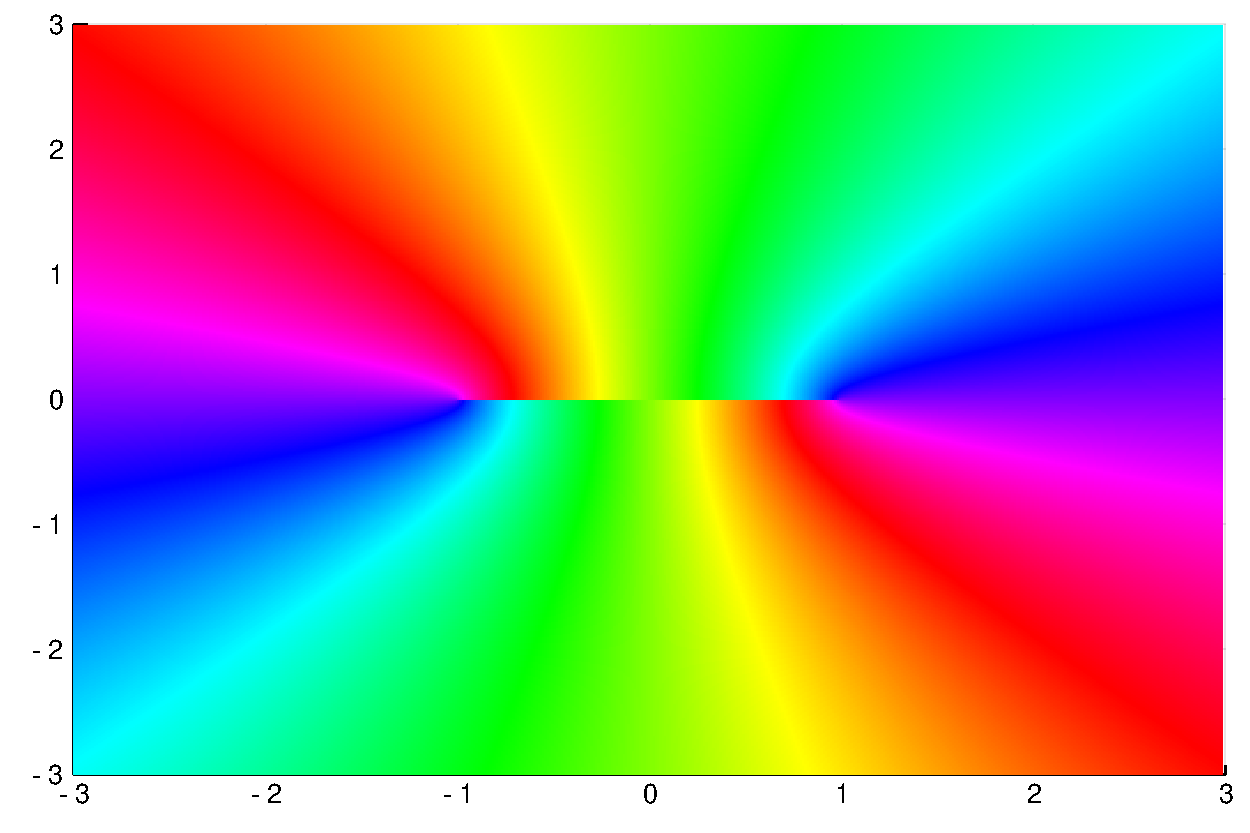
\includegraphics[width=\linewidth]{figures/Lecture23_1_1.pdf}

\subsection{Weighted Chebyshev log transform}
For classical orthogonal polynomials we can go a step further and relate the indefinite integrals to other orthogonal polynomials.

For example, recall that

\[
{\D\over \dx}[\sqrt{1-x^2} U_n(x)] = -{n+1 \over \sqrt{1-x^2}} T_{n+1}(x)
\]
in other words, 

\[
\int_x^1 {T_k(t) \over \sqrt{1-t^2}} \dt = -{\sqrt{1-x^2} U_{k-1}(x) \over k}
\]
Thus for $k=1,2,\ldots$,

\[
L_k(z) = -{1 \over n+1} \CC[\sqrt{1-\diamond^2} U_{k-1}](z)
\]
and

\[
{1 \over \pi} \int_{-1}^1 {T_k(x) \over \sqrt{1-x^2}}\log(z-x) \dx = {2 \I \over k}   \CC[\sqrt{1-\diamond^2} U_{k-1}](z)
\]
As we saw above, Cauchy transforms of OPs satisfy simple recurrences, and this relationship renders log transforms equally calculable. 

\subsection{Demonstration}
We first see how the Cauchy transform can be computed using forward recurrence if we know $C w(z)$. Here we consider the Chebyshev $T$ case:


\begin{lstlisting}
(*@\HLJLn{x}@*) (*@\HLJLoB{=}@*) (*@\HLJLnf{Fun}@*)(*@\HLJLp{()}@*)
(*@\HLJLn{w}@*) (*@\HLJLoB{=}@*) (*@\HLJLni{1}@*)(*@\HLJLoB{/}@*)(*@\HLJLnf{sqrt}@*)(*@\HLJLp{(}@*)(*@\HLJLni{1}@*)(*@\HLJLoB{-}@*)(*@\HLJLn{x}@*)(*@\HLJLoB{{\textasciicircum}}@*)(*@\HLJLni{2}@*)(*@\HLJLp{)}@*)
(*@\HLJLn{z}@*) (*@\HLJLoB{=}@*) (*@\HLJLnfB{0.1}@*)(*@\HLJLoB{+}@*)(*@\HLJLnfB{0.1}@*)(*@\HLJLn{im}@*)

(*@\HLJLn{n}@*) (*@\HLJLoB{=}@*) (*@\HLJLni{10}@*)
(*@\HLJLn{L}@*) (*@\HLJLoB{=}@*) (*@\HLJLnf{zeros}@*)(*@\HLJLp{(}@*)(*@\HLJLn{ComplexF64}@*)(*@\HLJLp{,}@*)(*@\HLJLn{n}@*)(*@\HLJLp{,}@*)(*@\HLJLn{n}@*)(*@\HLJLp{)}@*)
(*@\HLJLn{L}@*)(*@\HLJLp{[}@*)(*@\HLJLni{1}@*)(*@\HLJLp{,}@*)(*@\HLJLni{1}@*)(*@\HLJLp{]}@*) (*@\HLJLoB{=}@*) (*@\HLJLni{1}@*)
(*@\HLJLn{L}@*)(*@\HLJLp{[}@*)(*@\HLJLni{2}@*)(*@\HLJLp{,}@*)(*@\HLJLni{1}@*)(*@\HLJLp{]}@*) (*@\HLJLoB{=}@*) (*@\HLJLoB{-}@*)(*@\HLJLn{z}@*)
(*@\HLJLn{L}@*)(*@\HLJLp{[}@*)(*@\HLJLni{2}@*)(*@\HLJLp{,}@*)(*@\HLJLni{2}@*)(*@\HLJLp{]}@*) (*@\HLJLoB{=}@*) (*@\HLJLni{1}@*)
(*@\HLJLk{for}@*) (*@\HLJLn{k}@*)(*@\HLJLoB{=}@*)(*@\HLJLni{3}@*)(*@\HLJLoB{:}@*)(*@\HLJLn{n}@*)
    (*@\HLJLn{L}@*)(*@\HLJLp{[}@*)(*@\HLJLn{k}@*)(*@\HLJLp{,}@*)(*@\HLJLn{k}@*)(*@\HLJLoB{-}@*)(*@\HLJLni{1}@*)(*@\HLJLp{]}@*) (*@\HLJLoB{=}@*) (*@\HLJLoB{-}@*)(*@\HLJLn{z}@*)
    (*@\HLJLn{L}@*)(*@\HLJLp{[}@*)(*@\HLJLn{k}@*)(*@\HLJLp{,}@*)(*@\HLJLn{k}@*)(*@\HLJLoB{-}@*)(*@\HLJLni{2}@*)(*@\HLJLp{]}@*) (*@\HLJLoB{=}@*) (*@\HLJLn{L}@*)(*@\HLJLp{[}@*)(*@\HLJLn{k}@*)(*@\HLJLp{,}@*)(*@\HLJLn{k}@*)(*@\HLJLp{]}@*) (*@\HLJLoB{=}@*) (*@\HLJLni{1}@*)(*@\HLJLoB{/}@*)(*@\HLJLni{2}@*)
(*@\HLJLk{end}@*)

(*@\HLJLn{C}@*) (*@\HLJLoB{=}@*) (*@\HLJLn{L}@*) (*@\HLJLoB{{\textbackslash}}@*) (*@\HLJLp{[}@*) (*@\HLJLn{im}@*)(*@\HLJLoB{/}@*)(*@\HLJLp{(}@*)(*@\HLJLni{2}@*)(*@\HLJLnf{sqrt}@*)(*@\HLJLp{(}@*)(*@\HLJLn{z}@*)(*@\HLJLoB{-}@*)(*@\HLJLni{1}@*)(*@\HLJLp{)}@*)(*@\HLJLnf{sqrt}@*)(*@\HLJLp{(}@*)(*@\HLJLn{z}@*)(*@\HLJLoB{+}@*)(*@\HLJLni{1}@*)(*@\HLJLp{));}@*) (*@\HLJLni{1}@*)(*@\HLJLoB{/}@*)(*@\HLJLp{(}@*)(*@\HLJLni{2}@*)(*@\HLJLn{im}@*)(*@\HLJLp{);}@*) (*@\HLJLnf{zeros}@*)(*@\HLJLp{(}@*)(*@\HLJLn{n}@*)(*@\HLJLoB{-}@*)(*@\HLJLni{2}@*)(*@\HLJLp{)]}@*)

(*@\HLJLn{T\ensuremath{\_5}}@*) (*@\HLJLoB{=}@*) (*@\HLJLnf{Fun}@*)(*@\HLJLp{(}@*)(*@\HLJLnf{Chebyshev}@*)(*@\HLJLp{(),}@*) (*@\HLJLp{[}@*)(*@\HLJLnf{zeros}@*)(*@\HLJLp{(}@*)(*@\HLJLni{5}@*)(*@\HLJLp{);}@*)(*@\HLJLni{1}@*)(*@\HLJLp{])}@*)
(*@\HLJLnf{cauchy}@*)(*@\HLJLp{(}@*)(*@\HLJLn{T\ensuremath{\_5}}@*)(*@\HLJLoB{*}@*)(*@\HLJLn{w}@*)(*@\HLJLp{,}@*)(*@\HLJLn{z}@*)(*@\HLJLp{)}@*) (*@\HLJLp{,}@*) (*@\HLJLn{C}@*)(*@\HLJLp{[}@*)(*@\HLJLni{6}@*)(*@\HLJLp{]}@*)
\end{lstlisting}

\begin{lstlisting}
(0.14734333381379638 - 0.26445831594251407im, 0.14734333381379644 - 0.26445
83159425141im)
\end{lstlisting}


\textbf{Warning} This fails for large $n$ or large $z$:


\begin{lstlisting}
(*@\HLJLn{x}@*) (*@\HLJLoB{=}@*) (*@\HLJLnf{Fun}@*)(*@\HLJLp{()}@*)
(*@\HLJLn{w}@*) (*@\HLJLoB{=}@*) (*@\HLJLni{1}@*)(*@\HLJLoB{/}@*)(*@\HLJLnf{sqrt}@*)(*@\HLJLp{(}@*)(*@\HLJLni{1}@*)(*@\HLJLoB{-}@*)(*@\HLJLn{x}@*)(*@\HLJLoB{{\textasciicircum}}@*)(*@\HLJLni{2}@*)(*@\HLJLp{)}@*)
(*@\HLJLn{z}@*) (*@\HLJLoB{=}@*) (*@\HLJLni{5}@*)(*@\HLJLoB{+}@*)(*@\HLJLni{6}@*)(*@\HLJLn{im}@*)

(*@\HLJLn{n}@*) (*@\HLJLoB{=}@*) (*@\HLJLni{100}@*)
(*@\HLJLn{L}@*) (*@\HLJLoB{=}@*) (*@\HLJLnf{zeros}@*)(*@\HLJLp{(}@*)(*@\HLJLn{ComplexF64}@*)(*@\HLJLp{,}@*)(*@\HLJLn{n}@*)(*@\HLJLp{,}@*)(*@\HLJLn{n}@*)(*@\HLJLp{)}@*)
(*@\HLJLn{L}@*)(*@\HLJLp{[}@*)(*@\HLJLni{1}@*)(*@\HLJLp{,}@*)(*@\HLJLni{1}@*)(*@\HLJLp{]}@*) (*@\HLJLoB{=}@*) (*@\HLJLni{1}@*)
(*@\HLJLn{L}@*)(*@\HLJLp{[}@*)(*@\HLJLni{2}@*)(*@\HLJLp{,}@*)(*@\HLJLni{1}@*)(*@\HLJLp{]}@*) (*@\HLJLoB{=}@*) (*@\HLJLoB{-}@*)(*@\HLJLn{z}@*)
(*@\HLJLn{L}@*)(*@\HLJLp{[}@*)(*@\HLJLni{2}@*)(*@\HLJLp{,}@*)(*@\HLJLni{2}@*)(*@\HLJLp{]}@*) (*@\HLJLoB{=}@*) (*@\HLJLni{1}@*)
(*@\HLJLk{for}@*) (*@\HLJLn{k}@*)(*@\HLJLoB{=}@*)(*@\HLJLni{3}@*)(*@\HLJLoB{:}@*)(*@\HLJLn{n}@*)
    (*@\HLJLn{L}@*)(*@\HLJLp{[}@*)(*@\HLJLn{k}@*)(*@\HLJLp{,}@*)(*@\HLJLn{k}@*)(*@\HLJLoB{-}@*)(*@\HLJLni{1}@*)(*@\HLJLp{]}@*) (*@\HLJLoB{=}@*) (*@\HLJLoB{-}@*)(*@\HLJLn{z}@*)
    (*@\HLJLn{L}@*)(*@\HLJLp{[}@*)(*@\HLJLn{k}@*)(*@\HLJLp{,}@*)(*@\HLJLn{k}@*)(*@\HLJLoB{-}@*)(*@\HLJLni{2}@*)(*@\HLJLp{]}@*) (*@\HLJLoB{=}@*) (*@\HLJLn{L}@*)(*@\HLJLp{[}@*)(*@\HLJLn{k}@*)(*@\HLJLp{,}@*)(*@\HLJLn{k}@*)(*@\HLJLp{]}@*) (*@\HLJLoB{=}@*) (*@\HLJLni{1}@*)(*@\HLJLoB{/}@*)(*@\HLJLni{2}@*)
(*@\HLJLk{end}@*)

(*@\HLJLn{C}@*) (*@\HLJLoB{=}@*) (*@\HLJLn{L}@*) (*@\HLJLoB{{\textbackslash}}@*) (*@\HLJLp{[}@*) (*@\HLJLn{im}@*)(*@\HLJLoB{/}@*)(*@\HLJLp{(}@*)(*@\HLJLni{2}@*)(*@\HLJLnf{sqrt}@*)(*@\HLJLp{(}@*)(*@\HLJLn{z}@*)(*@\HLJLoB{-}@*)(*@\HLJLni{1}@*)(*@\HLJLp{)}@*)(*@\HLJLnf{sqrt}@*)(*@\HLJLp{(}@*)(*@\HLJLn{z}@*)(*@\HLJLoB{+}@*)(*@\HLJLni{1}@*)(*@\HLJLp{));}@*) (*@\HLJLni{1}@*)(*@\HLJLoB{/}@*)(*@\HLJLp{(}@*)(*@\HLJLni{2}@*)(*@\HLJLn{im}@*)(*@\HLJLp{);}@*) (*@\HLJLnf{zeros}@*)(*@\HLJLp{(}@*)(*@\HLJLn{n}@*)(*@\HLJLoB{-}@*)(*@\HLJLni{2}@*)(*@\HLJLp{)]}@*)

(*@\HLJLn{T\ensuremath{\_2}\ensuremath{\_0}}@*) (*@\HLJLoB{=}@*) (*@\HLJLnf{Fun}@*)(*@\HLJLp{(}@*)(*@\HLJLnf{Chebyshev}@*)(*@\HLJLp{(),}@*) (*@\HLJLp{[}@*)(*@\HLJLnf{zeros}@*)(*@\HLJLp{(}@*)(*@\HLJLni{20}@*)(*@\HLJLp{);}@*)(*@\HLJLni{1}@*)(*@\HLJLp{])}@*)

(*@\HLJLn{C}@*)(*@\HLJLp{[}@*)(*@\HLJLni{21}@*)(*@\HLJLp{],}@*) (*@\HLJLnf{cauchy}@*)(*@\HLJLp{(}@*)(*@\HLJLn{T\ensuremath{\_2}\ensuremath{\_0}}@*)(*@\HLJLoB{*}@*)(*@\HLJLn{w}@*)(*@\HLJLp{,}@*) (*@\HLJLn{z}@*)(*@\HLJLp{)}@*)
\end{lstlisting}

\begin{lstlisting}
(-2.591846965643171e6 - 48792.874011516105im, 0.0 + 8.834874115176436e-18im
)
\end{lstlisting}


Get around it by dropping the first row:


\begin{lstlisting}
(*@\HLJLn{L}@*)(*@\HLJLp{[}@*)(*@\HLJLni{2}@*)(*@\HLJLoB{:}@*)(*@\HLJLk{end}@*)(*@\HLJLp{,}@*)(*@\HLJLni{1}@*)(*@\HLJLoB{:}@*)(*@\HLJLk{end}@*)(*@\HLJLoB{-}@*)(*@\HLJLni{1}@*)(*@\HLJLp{]}@*)

(*@\HLJLn{C}@*) (*@\HLJLoB{=}@*) (*@\HLJLn{L}@*)(*@\HLJLp{[}@*)(*@\HLJLni{2}@*)(*@\HLJLoB{:}@*)(*@\HLJLk{end}@*)(*@\HLJLp{,}@*)(*@\HLJLni{1}@*)(*@\HLJLoB{:}@*)(*@\HLJLk{end}@*)(*@\HLJLoB{-}@*)(*@\HLJLni{1}@*)(*@\HLJLp{]}@*)(*@\HLJLoB{{\textbackslash}}@*) (*@\HLJLp{[}@*)(*@\HLJLni{1}@*)(*@\HLJLoB{/}@*)(*@\HLJLp{(}@*)(*@\HLJLni{2}@*)(*@\HLJLn{im}@*)(*@\HLJLp{);}@*) (*@\HLJLnf{zeros}@*)(*@\HLJLp{(}@*)(*@\HLJLn{n}@*)(*@\HLJLoB{-}@*)(*@\HLJLni{2}@*)(*@\HLJLp{)]}@*)

(*@\HLJLn{C}@*)(*@\HLJLp{[}@*)(*@\HLJLni{6}@*)(*@\HLJLp{]}@*)(*@\HLJLoB{-}@*) (*@\HLJLnf{cauchy}@*)(*@\HLJLp{(}@*)(*@\HLJLn{T\ensuremath{\_5}}@*)(*@\HLJLoB{*}@*)(*@\HLJLn{w}@*)(*@\HLJLp{,}@*) (*@\HLJLn{z}@*)(*@\HLJLp{)}@*)
\end{lstlisting}

\begin{lstlisting}
-3.072062106493749e-17 + 4.410018806364391e-17im
\end{lstlisting}


We can also use this technique for computing Hiblert transforms:


\begin{lstlisting}
(*@\HLJLn{x}@*) (*@\HLJLoB{=}@*) (*@\HLJLnfB{0.1}@*)

(*@\HLJLn{T}@*) (*@\HLJLoB{=}@*) (*@\HLJLnf{Fun}@*)(*@\HLJLp{(}@*)(*@\HLJLnf{Chebyshev}@*)(*@\HLJLp{(),[}@*)(*@\HLJLnf{zeros}@*)(*@\HLJLp{(}@*)(*@\HLJLn{n}@*)(*@\HLJLp{);}@*)(*@\HLJLni{1}@*)(*@\HLJLp{])}@*)
(*@\HLJLnf{hilbert}@*)(*@\HLJLp{(}@*)(*@\HLJLn{w}@*)(*@\HLJLoB{*}@*)(*@\HLJLn{T}@*)(*@\HLJLp{,}@*)(*@\HLJLn{x}@*)(*@\HLJLp{)}@*) (*@\HLJLp{,}@*) (*@\HLJLnf{Fun}@*)(*@\HLJLp{(}@*)(*@\HLJLnf{Ultraspherical}@*)(*@\HLJLp{(}@*)(*@\HLJLni{1}@*)(*@\HLJLp{),}@*) (*@\HLJLp{[}@*)(*@\HLJLnf{zeros}@*)(*@\HLJLp{(}@*)(*@\HLJLn{n}@*)(*@\HLJLoB{-}@*)(*@\HLJLni{1}@*)(*@\HLJLp{);}@*)(*@\HLJLni{1}@*)(*@\HLJLp{])(}@*)(*@\HLJLn{x}@*)(*@\HLJLp{)}@*)
\end{lstlisting}

\begin{lstlisting}
(0.5608031061203765, 0.5608031061203765)
\end{lstlisting}


And Log transforms:


\begin{lstlisting}
(*@\HLJLn{T\ensuremath{\_5}}@*) (*@\HLJLoB{=}@*) (*@\HLJLnf{Fun}@*)(*@\HLJLp{(}@*)(*@\HLJLnf{Chebyshev}@*)(*@\HLJLp{(),}@*) (*@\HLJLp{[}@*)(*@\HLJLnf{zeros}@*)(*@\HLJLp{(}@*)(*@\HLJLni{5}@*)(*@\HLJLp{);}@*)(*@\HLJLni{1}@*)(*@\HLJLp{])}@*)
(*@\HLJLn{U\ensuremath{\_4}}@*) (*@\HLJLoB{=}@*) (*@\HLJLnf{Fun}@*)(*@\HLJLp{(}@*)(*@\HLJLnf{Ultraspherical}@*)(*@\HLJLp{(}@*)(*@\HLJLni{1}@*)(*@\HLJLp{),}@*) (*@\HLJLp{[}@*)(*@\HLJLnf{zeros}@*)(*@\HLJLp{(}@*)(*@\HLJLni{4}@*)(*@\HLJLp{);}@*)(*@\HLJLni{1}@*)(*@\HLJLp{])}@*)
(*@\HLJLn{x}@*) (*@\HLJLoB{=}@*) (*@\HLJLnf{Fun}@*)(*@\HLJLp{()}@*)
(*@\HLJLn{L\ensuremath{\_5}}@*) (*@\HLJLoB{=}@*) (*@\HLJLn{z}@*)(*@\HLJLoB{->}@*)(*@\HLJLnf{sum}@*)(*@\HLJLp{(}@*)(*@\HLJLn{T\ensuremath{\_5}}@*)(*@\HLJLoB{/}@*)(*@\HLJLnf{sqrt}@*)(*@\HLJLp{(}@*)(*@\HLJLni{1}@*)(*@\HLJLoB{-}@*)(*@\HLJLn{x}@*)(*@\HLJLoB{{\textasciicircum}}@*)(*@\HLJLni{2}@*)(*@\HLJLp{)}@*) (*@\HLJLoB{*}@*) (*@\HLJLnf{log}@*)(*@\HLJLp{(}@*)(*@\HLJLn{z}@*)(*@\HLJLoB{-}@*)(*@\HLJLn{x}@*)(*@\HLJLp{))}@*)(*@\HLJLoB{/}@*)(*@\HLJLn{\ensuremath{\pi}}@*)

(*@\HLJLnf{L\ensuremath{\_5}}@*)(*@\HLJLp{(}@*)(*@\HLJLn{z}@*)(*@\HLJLp{),}@*) (*@\HLJLni{2}@*)(*@\HLJLn{im}@*)(*@\HLJLoB{*}@*)(*@\HLJLnf{cauchy}@*)(*@\HLJLp{(}@*)(*@\HLJLnf{sqrt}@*)(*@\HLJLp{(}@*)(*@\HLJLni{1}@*)(*@\HLJLoB{-}@*)(*@\HLJLn{x}@*)(*@\HLJLoB{{\textasciicircum}}@*)(*@\HLJLni{2}@*)(*@\HLJLp{)}@*)(*@\HLJLoB{*}@*)(*@\HLJLn{U\ensuremath{\_4}}@*)(*@\HLJLp{,}@*)(*@\HLJLn{z}@*)(*@\HLJLp{)}@*)(*@\HLJLoB{/}@*)(*@\HLJLni{5}@*)
\end{lstlisting}

\begin{lstlisting}
(6.576121814966233e-8 - 2.0389718362285204e-7im, 6.576121814966217e-8 - 2.0
389718362285196e-7im)
\end{lstlisting}



\end{document}
